% !TeX encoding = UTF-8
% !TeX spellcheck = es_ES
% !TeX root = ComponentCatalog.tex
%!TEX root=ComponentCatalog.tex
\subsection{Grafico}
\begin{table}[H]
    \centering
    \renewcommand\theadfont{\bfseries}
    \setlength{\tabcolsep}{10pt}
    \renewcommand{\arraystretch}{1.5}

    \begin{tabular}{|c|c|c|c|c|}
        \beginConnectorTable{TFT}
        \multirow{4}{*}{\makecell{1.8 SPI \\  }}
        \connectordata{
            \begin{scope}
                \clip (0,0) rectangle  +(3,1.5);
                \node[inner sep=0pt] at (1.5,0.8)
                    {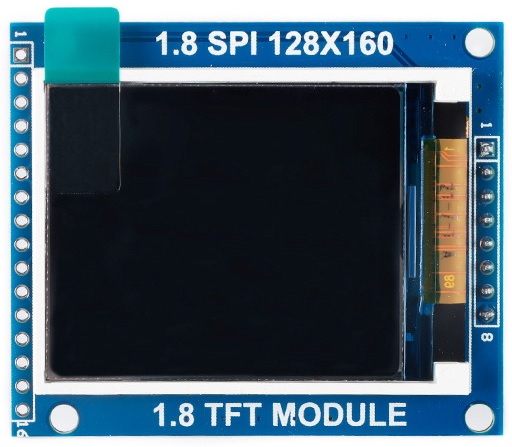
\includegraphics[scale=0.16]{pictures/1.8SPITFT.jpg}};
            \end{scope}
        }{
            \draw (0,0) rectangle (3,1.5) ;
        }{Aliexpress}{1.8 SPI TFT} {5V} {50mA} 
        
        \connectorinfo{Chip}{ST7735B}{
            \tabitem Tiene para una SD
        }
        \multirow{4}{*}{\makecell{0.96 I2C \\  }}
        \connectordata{
            \begin{scope}
                \clip (0,0) rectangle  +(3,1.5);
                \node[inner sep=0pt] at (1.5,0.8)
                    {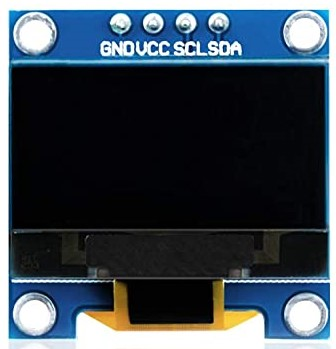
\includegraphics[scale=0.16]{pictures/0.96I2CTFT.jpg}};
            \end{scope}
        }{
            \draw (0,0) rectangle (3,1.5) ;
        }{Amazon}{0.96 I2C TFT} {5V} {50mA} 
        
        \connectorinfo{Chip}{SSD 1306}{
            \tabitem Color Blanco
        }
        \hline
        \connectorblockinfo{Uso}{Dcc Decoder Config}
        \connectorblockinfo{Ubicacion}{TT-Tren}
    \end{tabular}
    \caption{Displays Graficos}
    \label{tab:GraphicDisplay}
\end{table}